\documentclass[12pt]{article}
\usepackage{amsfonts, amssymb, amsmath, amsthm}
\usepackage[margin=1in]{geometry}
\usepackage{tikz}

\title{Explainer: Problem 3 (Rudin 6.18) --- Same Range, Different Lengths}
\author{}
\date{}

\begin{document}
\maketitle

\section*{The three curves}
All three map $[0, 2\pi]$ into the unit circle in $\mathbb{C}$:
\begin{align*}
\gamma_1(t) &= e^{it} && \text{(once around, counterclockwise)} \\
\gamma_2(t) &= e^{2it} && \text{(twice around)} \\
\gamma_3(t) &= e^{2\pi i t \sin(1/t)} && \text{(wild oscillation near $t = 0$)}
\end{align*}

\section*{Same range, different curves}
A \textbf{curve} is a \emph{map}, not just its image. Two curves with identical image (the unit circle here) can have very different ``lengths'' because length counts \emph{how many times} you traverse. $\gamma_2$ goes around twice, so length $= 4\pi = 2 \cdot (2\pi)$.

\begin{center}
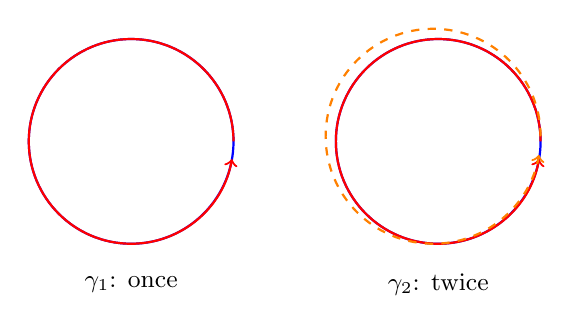
\begin{tikzpicture}[scale=1.3]
  \draw[thick, blue] (0,0) circle (1);
  \draw[->, red, thick] (1,0) arc (0:350:1);
  \node at (0, -1.4) {\small $\gamma_1$: once};
  \begin{scope}[xshift=3cm]
    \draw[thick, blue] (0,0) circle (1);
    \draw[->, red, thick] (1,0) arc (0:350:1);
    \draw[->, orange, thick, dashed] (1, 0.05) arc (0:350:1.05);
    \node at (0, -1.4) {\small $\gamma_2$: twice};
  \end{scope}
\end{tikzpicture}
\end{center}

\section*{Length of a curve}
Length $= \sup_P \sum_{i} |\gamma(t_i) - \gamma(t_{i-1})|$, the supremum of polygonal lengths over partitions $P$ of $[a,b]$. A curve is \textbf{rectifiable} if this sup is finite.

For smooth curves there's a formula: length $= \int_a^b |\gamma'(t)|\, dt$. Both $\gamma_1$ and $\gamma_2$ are smooth with $|\gamma_j'| = j$, giving $j \cdot 2\pi$.

\section*{Why $\gamma_3$ is not rectifiable}
Near $t = 0$, the function $t \sin(1/t)$ oscillates wildly. The exponent $2\pi i t \sin(1/t)$ makes $\gamma_3$ sweep around the circle infinitely often in any neighborhood of $t = 0$, and these sweeps don't shrink fast enough.

\begin{center}
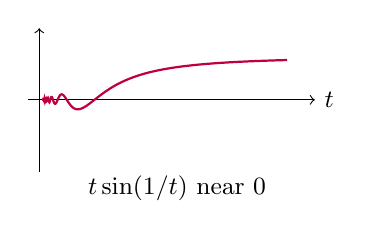
\begin{tikzpicture}[scale=0.7]
  \draw[->] (-0.2, 0) -- (5, 0) node[right] {\small $t$};
  \draw[->] (0, -1.3) -- (0, 1.3);
  \draw[domain=0.05:4.5, samples=500, smooth, thick, purple] plot (\x, {\x/4 * sin(180/\x)});
  \node at (2.5, -1.6) {\small $t \sin(1/t)$ near $0$};
\end{tikzpicture}
\end{center}

\textbf{Strategy:} Find a sequence of times $t_n \to 0$ where $t_n \sin(1/t_n)$ hits half-integer values (so $\gamma_3(t_n)$ alternates $\pm 1$ on the circle). Then the polygonal sum $\sum |\gamma_3(t_n) - \gamma_3(t_{n+1})|$ accumulates $\geq 2$ each step, infinitely many times --- diverges.

\textbf{Hint:} Try $t_n$ such that $1/t_n \sin(1/t_n) = $ integer, or pick $t_n = 1/(n\pi/2)$ type values to make $\sin(1/t_n) = \pm 1$ and catch the extremes of the oscillation.

\end{document}
